% !TeX root = ./00.ppgcc-2020.tex

% \chapter{Implementação}\label{cha:implementacao}

% % procedimento experimental previamente definido de ambos, \mfog e da
% % implementação original do algoritmo MINAS, e comparadas.

% % !TeX root = ./00.ppgcc-2020.tex

\subsection{Implementações Preliminares}\label{sec:resultados}

No desenvolvimento parcial desta pesquisa, algumas experimentações e algumas
ferramentas de teste já foram desenvolvidas.
Aspectos desses desenvolvimentos são descritos a seguir.
% obrigado hélio.

\subsubsection{Implementação com \python e \kafka}

A primeira implementação e avaliação do \mfog realizada foi construída sobre a
linguagem \python com o sistema de fila de mensagens \kafka e a respectiva
biblioteca de conexão.
A escolha desse conjunto para a implementação ocorreu \hlhl{devido à ampla}
disponibilidade de bibliotecas de aprendizagem de máquina no ecossistema
\python e, à simplicidade geral da linguagem.
Na implementação desenvolvida, o sistema \kafka recebe mensagens e as armazena
em tópicos distribuídos em partições replicadas em nós de um \cluster,
gerenciados por um nó mestre e suportados pelo serviço de gerenciamento de
configuração distribuída \emph{Apache ZooKeeper}.
A aplicação \emph{Python} consome eventos através da interface \emph{Consumer API},
que expõe a distribuição através da associação de um consumidor às partições
mantidas pelo \kafka.

Para essa implementação, havia a hipótese de que a distribuição de
mensagens gerenciada pelo \kafka
se estenderia a processos consumidores, efetivamente distribuindo o volume de
mensagens entre eles igualmente.
No entanto, a hipótese foi refutada nos experimentos realizados.
Os experimentos em questão foram compostos de 8 processos consumidores, um
processo produtor, uma instância \kafka com 8 partições em seu tópico principal
e uma instância \emph{Apache ZooKeeper} associada à instância \kafka.
% A hipótese era que, como o número de partições igualava o número de consumidores,
% cada consumidor associaria-se a uma partição, distribuindo os dados igualmente
% entre os consumidores para a paralelização a execução.
A hipótese foi refutada quando observou-se que o número de
mensagens consumidas por um dos 8 processos representava a maioria (mais de
80\%) do volume introduzido no sistema, o restante sendo distribuído entre
outros 3 processos e o restante dos processos não recebia nenhuma mensagem.
Portanto, a iniciativa de implementar o algoritmo MINAS em \python com \kafka e
atingir os objetivos de distribuição falhou, o que levou à reconsideração das
plataformas escolhidas.

\subsubsection{Implementação com \flink}

% \nota{citar ferramentas e a escolha só depois do python e kafka}
% \nota{entre flink e spark, outro grupo de pesquisa já está explorando spark}

A segunda alternativa explorada teve por inspiração o trabalho de
\citeonline{Viegas2019} e, como outro grupo de pesquisa já estava explorando
o algoritmo na plataforma \emph{Apache Spark}, a segunda implementação
foi baseada na plataforma \flink.

A plataforma \flink tem modelos de processamento tanto de fluxos como em lotes.
O modelo em lotes é implementado como extensão do modelo de fluxos e, apesar
de não ser foco desse trabalho, mostrou-se útil para a construção do \offline,
já que o conjunto consumido por esse módulo é limitado.

Um desafio encontrado durante o desenvolvimento da implementação do \mfog foi a falta
de bibliotecas na plataforma \flink que disponibilizem versões adaptadas
à plataforma de algoritmos base para o algoritmo MINAS.
Em especial, a ausência dos algoritmos \emph{K-means} e \emph{CluStream}
gerou carga imprevista sobre o processo de desenvolvimento
resultando no atraso do processo de desenvolvimento.

Esta implementação segue a arquitetura descrita na \refsec{descricao} e as
avaliações e resultados esperados descritos neste \refcap{proposta}
referem-se à implementação do \mfog na plataforma \flink.

% % !TeX root = ./00.ppgcc-2020.tex

\section{Implementação com MPI}

The original MINAS algorithm has a companion unpublished implementation (\refminas)
written in Java using MOA library base algorithms such as K-means and CluStream,
but our implementation only used K-means.
Another difference between \refminas and \mfog is the calculus of the cluster radius 
from the distances of elements forming the cluster and the cluster's center.
\refminas uses the maximum distance while \mfog uses the standard deviation
of all distances as described in \cite{Faria2016minas}.

\newcommand{\val}{$\vec{v}\,$\xspace}
The stream formats for input and output are also of note.
As input, the algorithm takes samples (\val), which are a sequence of numbers
with dimension $d$.
In addition to \val, for both training and evaluation, the class
identifier is provided as a single character, along with a unique item identifier
(\emph{uid}), which can otherwise be determined from the sample index in the stream.

As its output, the algorithm returns the original sample \val followed by the
assigned label. Adjustments can easily be made to provide the output results as
a tuple containing \emph{uid} and the assigned label.

% - Reprocessamento dos exemplos utilizados para atualização do modelo:
%   - Muda o comportamento do operador de fluxo de `Map` para `Flatmap`, ou seja,
%     requer outro fluxo de saída para a transmissão de padrões novidade (alarmes);
%   - Para reclassificação a definição de raio é modificada de `r = f * σ` (fator
%     multiplicando desvio padrão) para `r = max(distance)` (distância máxima);
%   - Passível da crítica de *overfitting*. Isto é, este processo pode
%     inflar a métrica de precisão;
%   - **Solução:** *em aberto*;


\begin{algorithm}[htb]
% {\scriptsize
% \begin{multicols}{2}
    % \SetAlgoVlined
    \SetKwProg{Function}{Function}{:}{}
    \SetKwFor{With}{with}{}{}
    \SetKw{continue}{continue}
    % 
    \SetKwData{MEPC}{MEPC}
    \SetKwData{NF}{NF}
    \SetKwData{mpiSize}{mpiSize}
    \SetKwData{mpiRank}{mpiRank}
    \SetKwData{EndOfStream}{EndOfStream}
    % 
    \SetKwInOut{KwParams}{Parameters}
    \KwParams{mpiNodeRank as \mpiRank}
    % 
    \SetKwFunction{Mfog}{Mfog}
    \SetKwFunction{Sampler}{Sampler}
    \SetKwFunction{Classifier}{Classifier}
    \SetKwFunction{Detector}{Detector}
    \SetKwFunction{modelReceiver}{modelReceiver}
    % 
    \SetKwFunction{typeOf}{typeOf}
    % 
    \SetKwFunction{Thread}{Thread}
    \SetKwFunction{Lock}{Lock}
    \SetKwFunction{readLock}{readLock}
    \SetKwFunction{writeLock}{writeLock}
    % 
    \SetKwFunction{receive}{receive}
    \SetKwFunction{send}{send}
    \SetKwFunction{broadcast}{broadcast}
    % 
    \SetKwFunction{nearestCluster}{nearestCluster}
    \SetKwFunction{NoveltyDetection}{NoveltyDetection}
    \SetKwFunction{handleModelSleep}{handleModelSleep}
    \SetKwFunction{removeOldSamples}{removeOldSamples}
    \SetKwFunction{now}{now}
    % 
    \KwIn{ModelSet, Sample Stream}
    % \KwOut{Classified Stream as $out$}
    % 
    \Function{\Mfog{ModelStream, InputStream, OutputStream}}{
        ModelSet = $\emptyset$\;
        ModelSetLock = \textbf{new} \Lock()\;
        \eIf(\emph{root}){\mpiRank == 0}{
            \textbf{new} \Thread(\Detector, [OutputStream, ModelSet, ModelSetLock])\;
            \Sampler(InputStream, ModelSet, ModelSetLock)\;
        }(\emph{leaf}){
            \textbf{new} \Thread(\modelReceiver, [ModelSet, ModelSetLock])\;
            \Classifier(ModelSet, ModelSetLock)\;
        }
    }
\caption{MFOG: main MPI entry-point.}
\label{alg:MFOG}
\end{algorithm}

\begin{algorithm}[htb]
    \SetKwFor{With}{with}{}{}
    \SetKw{continue}{continue}
    % 
    \SetKwData{MEPC}{MEPC}
    \SetKwData{NF}{NF}
    \SetKwData{mpiSize}{mpiSize}
    \SetKwData{mpiRank}{mpiRank}
    \SetKwData{EndOfStream}{EndOfStream}
    % 
    \SetKwProg{Function}{Function}{:}{}
    \Function{\Classifier{ModelSet, ModelSetLock}}{
        \While{ True }{
            sampe = \receive(SampleType, root)\;
            \lIf{sample == \EndOfStream}{\textbf{break}}
            sample.label = unknown\;
            \With{\readLock(ModelSetLock)}{
                (distance, cluster) = \nearestCluster(sample, ModelSet)\;
            }
            \If{distance $<$ cluster.radius}{
                sample.label = cluster.label\;
            }
            \send(root, SampleType, sample)\;
        }
    }
%     \label{alg:MFOG-classifier}
%     \caption{MFOG: Classifier task.}
% \end{algorithm}
% \begin{algorithm}
    % \SetKwProg{algorithm}{algorithm}{:}{}
    \SetKwFor{With}{with}{}{}
    \SetKw{continue}{continue}
    % 
    \SetKwData{MEPC}{MEPC}
    \SetKwData{NF}{NF}
    \SetKwData{mpiSize}{mpiSize}
    \SetKwData{mpiRank}{mpiRank}
    \SetKwData{EndOfStream}{EndOfStream}
    % 
    \SetKwProg{Function}{Function}{:}{}
    \Function{\modelReceiver{ModelSet, ModelSetLock}}{
        \While{ True }{
            cl = \receive(ClusterType, root)\;
            \lIf{cl == \EndOfStream}{\textbf{break}}
            \With{writeLock(ModelSetLock)}{
                ModelSet = ModelSet $\cup$ cl\;
            }
        }
    }
    % \label{alg:MFOG-model}
    % \caption{MFOG: model receiver task.}
\caption{MFOG Leaf Tasks: Model Receiver and Classifier.}
\label{alg:MFOG-leaf}
\end{algorithm}
\begin{algorithm}[htb]
    \SetKwFor{With}{with}{}{}
    \SetKw{continue}{continue}
    % 
    \SetKwData{MEPC}{MEPC}
    \SetKwData{NF}{NF}
    \SetKwData{mpiSize}{mpiSize}
    \SetKwData{mpiRank}{mpiRank}
    \SetKwData{EndOfStream}{EndOfStream}
    \SetKwInOut{KwParams}{Parameters}
    \KwParams{mpiClusterSize as \mpiSize}
    \SetKwProg{Function}{Function}{:}{}
    \Function{\Sampler{InputStream, ModelSet, ModelSetLock}}{
        % ModelSet = read()\;
        % broadcast(ModelSet)\;
        dest = 1\;
        \ForEach{ sample from InputStream }{
            \If{\typeOf(sample) is Cluster}{
                \broadcast(ClusterType, sample, root)\;
                \With{\writeLock(ModelSetLock)}{
                    ModelSet = ModelSet $\cup$ sample\;
                }
                \continue\;
            }
            % sample.label = unknown\;
            \send(dest, SampleType, sample)\;
            dest = dest $+ 1$\;
            \lIf{dest $>$ \mpiSize}{dest = 1}
        }
    }

%     \label{alg:MFOG-sampler}
%     \caption{MFOG: sampler Module.}
% \end{algorithm}
% \begin{algorithm}
    \SetKwProg{algorithm}{algorithm}{:}{}
    \SetKwFor{With}{with}{}{}
    \SetKw{continue}{continue}
    % 
    \SetKwData{cleaningWindow}{cleaningWindow}
    \SetKwFunction{removeOldSamples}{removeOldSamples}
    \SetKwData{noveltyDetectionTrigger}{noveltyDetectionTrigger}
    \SetKwData{MEPC}{MEPC}
    \SetKwData{NF}{NF}
    \SetKwData{mpiSize}{mpiSize}
    \SetKwData{mpiRank}{mpiRank}
    \SetKwData{EndOfStream}{EndOfStream}

    \KwParams{\cleaningWindow, \noveltyDetectionTrigger}

    \SetKwProg{Function}{Function}{:}{}
    \Function{\Detector{OutputStream, ModelSet, ModelSetLock}}{
        lastCleanup $\leftarrow 0$\;
        \While{ True }{
            sampe = \receive(SampleType, any)\;
            \lIf{sample == \EndOfStream}{\textbf{break}}
            % $out \leftarrow$ sample\;
            OutputStream.append(sample)\;
            \If{sample.label == unknown}{
                UnknownSet = UnknownSet $\cup$ sample\;
                \If{$|\;UnknownSet\;| \geq$ \noveltyDetectionTrigger}{
                    novelties = \NoveltyDetection(ModelSet, *UnknownSet)\;
                    \With{\writeLock(ModelSetLock)}{
                        ModelSet = ModelSet $\cup$ novelties\;
                    }
                    \ForEach{ cl in novelties }{
                        \broadcast(ClusterType, cl, root)\;
                    }
                }
                \If{ sampe.uid $ > $ ( lastCleanup $ + $ \cleaningWindow )}{
                    UnknownSet $\leftarrow$ \removeOldSamples(UnknownSet, lastCleanup)\;
                    lastCleanup $ \leftarrow $ sampe.uid\;
                }
            }
        }
    }
    % \label{alg:MFOG-detector}
    % \caption{MFOG: detector task.}
\caption{MFOG Root Tasks: Sampler and Detector.}
\label{alg:MFOG-root}
\end{algorithm}

For evaluation purposes, an \mfog implementation was made using MPI (\emph{Open
MPI 4.0.4}).
The program is organized in a single program multiple data (SPMD)
programming model, so a single version of the \mfog program was initiated on all
nodes, being that one of them would perform the root role, while the others ran
as leaves, the program entry point is illustrated on Algorithm \ref{alg:MFOG}.
On the root process, a sampler thread is responsible for distributing the
sampled flow information (\val) to the classifier nodes, using a round-robin
load balancing scheme.
The other thread on the root process is responsible for receiving the
classification results and for processing the unknown samples in the search for
novelties.
The root process functions are illustrated in Algorithm \ref{alg:MFOG-root}.
Each leaf node runs a model adjustment thread and multiple (up to the number of
cores) classifier threads. The leaf tasks are illustrated in Algorithm
\ref{alg:MFOG-leaf}.
The overall sequence of interactions is shown in Figure \ref{fig:mfog-mpi-life}.

\begin{figure}[htb]
  \centerline{
    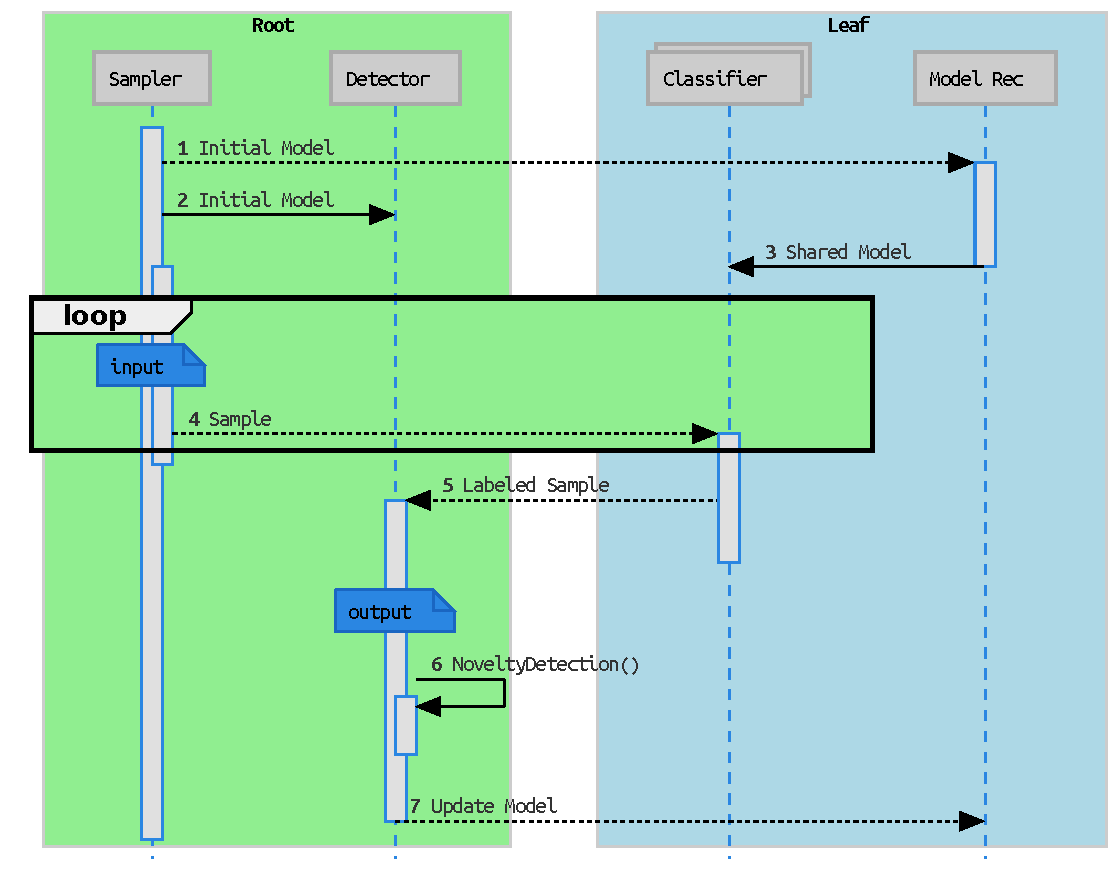
\includegraphics[width=0.75\linewidth,page=1]{figures/lifecycle-uml-svg.pdf}
  }
  \caption{\mfog life line overview.}
  \label{fig:mfog-mpi-life}
\end{figure}


\chapter{Experimentos e Resultados}\label{cha:results}

% !TeX root = ./00.ppgcc-2020.tex

\section{Ambiente de Teste}\label{sec:ambiente}

Com o objetivo de avaliar esta proposta e averiguar os efeitos da distribuição
da detecção de novidades em um cenário \iot, construiu-se um ambiente
experimental de névoa.

Este ambiente é composto por três computadores de única placa (\emph{Single
Board Computer}) modelo Raspberry Pi 3 model B, equipados com o SoC
(\emph{system-on-chip} - sistema em um chip) de arquitetura ARM \emph{BCM2837} com
$4$ núcleos de processamento à frequência de $1.2\,GHz$, $32\,kB$ e $512\,kB$ de
memória \emph{cache} nível 1 e 2 respectivamente, $1\,GB$ de memória RAM,
armazenamento em cartão SD e conectados por rede cabeada \emph{Ethernet}.
% Switch
% Hélio:
%    Há algo estranho na descrição dos nós; parece que você está misturando nós e cores.
%    Talvez seja mais claro falar do número de nós, ao invés dos cores...
% ficou melhor!

A ideia central é criar um cluster simples simulando \emph{gateway} de uma rede
\iot com recursos limitados.
Este cluster armazenou todo o código-fonte, binários (compilados no mesmo cluster) e
\dataset.
Nesta configuração, o \dataset é armazenado no cartão SD do nó raiz e é lido para
cada execução do experimento.
Todos os experimentos foram executados neste cluster para isolamento de outras
variações imprevistas e para garantir que as comparações seriam justas com
\emph{software} e \emph{hardware} constante.

% The idea was to create a simple cluster simulating an \iot network with
% constrained resources at the edge of the network.
% This cluster stored all source code, binaries (compiled and linked in place) and
% data sets.
% In our setup, the data set is stored in the root's node SD card and is read for
% each experiment.
% All experiments were executed in this cluster for isolation of otherwise
% unforeseen variations and for safe software comparison with constant hardware.
% data sets, being accessed via our laboratory network over Secure Shell (SSH).

O \dataset \emph{Kyoto 2006+}\footnote{Disponível em
\url{http://www.takakura.com/Kyoto\_data/}.}, tráfego das \emph{Honeypots} da
Universidade de Kyoto, é a referência de um cenário real para este trabalho.
% será que é o ``foco''? Talvez é a ``referência de um cenário real''...(?)
Este \dataset contém dados ainda representativos (até 2015) e as característica
desejáveis de um conjunto de dados (realismo, validade, etiquetas previamente
definidas, alta variabilidade, reprodutibilidade e disponibilidade pública) são
atendidas \cite{KyotoDataset,Song2011kyoto}.

O segmento utilizado deste \dataset é o de Dezembro de 2015, contendo $7\:865\:245$ instâncias.
Deste segmento, são mantidas apenas instâncias associadas a tráfego normal ou
a ataques conhecidos, identificados por \nids que tenham mais de $10\,000$ instâncias
para significância, como feito previamente por \citeonline{Cassales2019}.
% , this removes 46,390 instances. TODO: revisar, pois 7M != 700K.
As instâncias mantidas são normalizadas para que o valor de cada característica
original (como endereço IP, duração do fluxo, serviço) seja transposta para o
intervalo Real $[0, 1]$.

O conjunto resultante da operação recém descrita é então dividido em dois
conjuntos, treinamento e teste.
Para avaliar a detecção de ataques, o conjunto treinamento é composto apenas de
tráfego normal, contendo $72\:000$ instâncias.
O conjunto de teste possui $653\:457$ instâncias, sendo elas
$206\:278$ instâncias com classe ``$N$'' (normal) e
$447\:179$ instâncias com classe ``$A$'' (ataque).
%
% Não entendi essa questão de filtrar apenas os ``normal'' class no training set... Hélio
% acho que fez sentido... detectar o que não se aproxima de normal como novidade...

Destaca-se que essa manipulação do \dataset causa \emph{Overfitting} para a classe
normal e \emph{under-fitting} para a classe ataque, pois o sistema primeiro
precisa detectar um padrão novidade para então adicionar ao modelo.
%O foco deste trabalho não é a otimização da detecção de intrusão é contexto de validar metodologia de construcao do \mfog - distribuição e paralelismo em ambiente em \fog.
Como o foco deste trabalho é na arquitetura e metodologia de paralelização e
distribuição em névoa, a otimização do processo de detecção de intrusão não foi
abordada, deixando a questão de escolha do \dataset e do processo de sua manipulação
 em aberto.

Quanto aos parâmetros do algoritmo \minas, ilustrados na Figura
\ref{fig:params}, os valores foram escolhidos por \hlke{serem valores comuns para o
algoritmo presentes na literatura} \cite{Faria2013Minas,Faria2016minas} e na
implementação de referência \refminas \cite{Faria2013source}.
Os parâmetros que não tem valores comuns na literatura foram escolhidos e ajustados até os
os resultados obtidos se aproximarem aos resultados da implementação de referência \refminas.

\begin{figure}[htb]
  \centering
  \begin{lstlisting}
    MinasParams minasParams = {
      .k=100, .dim=22, .precision=1.0e-08,
      .radiusF=0.25, .minExamplesPerCluster=20, .noveltyF=1.4,
      .thresholdForgettingPast = 10000,
    };
  \end{lstlisting}
  \caption{Parâmetros do algoritmo \minas.}
  \label{fig:params}
\end{figure}

Os parâmetros utilizados da literatura são
\texttt{k}, que é o número de \mclusters gerados pelo algoritmo de agrupamento,
\texttt{minExamplesPerCluster}, que indica o número mínimo de exemplos para um
\mcluster válido (representatividade) e,
\texttt{thresholdForgettingPast}, que estabelece o limite para remoção de exemplos do conjunto de
desconhecidos.

Os parâmetros escolhidos por aproximação de resultados são:
\texttt{precision}, que é o valor limite para melhora na distância global reduzindo as 
iterações no algoritmo de agrupamento (otimização),
\texttt{radiusF}, que corresponde ao fator que multiplica o desvio padrão das distâncias entre o
centro e cada exemplo formador do novo \mcluster definindo o raio do \mcluster
e,
\texttt{noveltyF}, que é o fator que multiplica o desvio padrão das distâncias do
\mcluster mais próximo distinguindo um novo padrão entre extensão e novidade.

% (k, minExamplesPerCluster, noveltyF, thresholdForgettingPast)
% (precision, radiusF)

% Para realização dos experimentos, diversas configurações de ambientes são
% propostas.
% Os ambientes selecionados são: local, 
% \notahl{o que muda na paralelização e na \textbf{distribuição} de instâncias
% do módulo \textbf{classificador}?}
% \hlhl{nuvem e névoa}.
% As configurações consistem na distribuição de módulos da implementação \mfog
% sendo executadas em combinações de ambientes nuvem e névoa com variada
% quantidade de nós.
  % dá-lhe Yoda! Hélio

% O ambiente local é composto por um único nó computacional, consistindo de um
% computador pessoal equipado com um processador de 8 núcleos, $16GB$ de memória e
% armazenamento em estado sólido (SSD) usado para o desenvolvimento e referência
% em comparações.
% O ambiente nuvem é provido pela utilização da infraestrutura de nuvem da
% Universidade Federal de São Carlos (Cloud{@}UFSCar\footnote{Disponível em
% \url{http://portalcloud.ufscar.br/servicos}}).
% O ambiente de névoa (\fog) é composto por computadores de única placa
% (\emph{Single Board Computer}) equipados com processador de arquitetura ARM de 4
% núcleos, $1GB$ de memória, armazenamento em cartão SD (\emph{SD-card}) e
% conectados por rede sem fio.

% A combinação de diferentes formas de distribuição dos nós tem por objetivo \hlhl{demonstrar padrões de
% latência} e qualidade que podem afetar implantações em ambientes reais que não
% são geralmente destacados quando os experimentos são realizados em um único
% nó ou ambiente.

% Faz parte também do ambiente de teste os conjuntos de dados (\datasets)
% \emph{KDD99}
% % \hlfa{e \emph{Kyoto 2006+}}
% e \emph{Kyoto 2006+}
% que foram selecionados por motivos distintos.

% O \dataset \emph{Kyoto 2006+} é o foco deste trabalho, pois contém dados ainda
% representativos (até 2015) e as característica desejáveis de um conjunto de
% dados (realismo, validade, etiquetas previamente definidas, alta variabilidade,
% reprodutibilidade e disponibilidade pública) são atendidas
% \cite{KyotoDataset,Song2011kyoto}.

% O \dataset \emph{KDD99} é amplamente utilizado em trabalhos de detecção de
% anomalia.
% Porém, como não possui mais a característica de realismo, uma vez que foi
% construído em 1998, neste trabalho o \dataset \emph{KDD99} é utilizado somente
% para que o leitor possa comparar com outros trabalhos
% \cite{Tavallaee2009,Protic2018KddKyoto}.

% Os dois \datasets mencionados e outros abordados em discussão e avaliados como
% relevantes são

% Por exemplo, o KDD original tem 41 atributos. A base é rotulada para 24
% tipos de ataques divididos em 4 grupos: DOS ...
% 
% O paper que analisou a fundo o KDD99 foi este: 
% 
% M. Tavallaee, E. Bagheri, W. Lu, and A. Ghorbani, “A detailed analysis
% of the KDD Cup 1999 data set,” in Proc. 2nd IEEE Symp. Comput. Intell.
% Secur. Defense Appl., 2009, pp. 1–6.
% 
% Qual é o defeito dele? tem muitos dados replicdos tanto na base de
% treinamento quento na de teste, o que gera viés nos resultados. Para
% resolver isso propuseram o NSL-KDD que é um subconjunto do KDD que evita
% esse problema

% \notake{
%   CICIDS2017 {https://www.unb.ca/cic/datasets/ids-2017.html} e
%   ISCXTor2016 {https://github.com/ahlashkari/CICFlowMeter}
% }
% \notafa{Uma sugestão seria usar datasets artificiais também a fim de avaliar
% outras caracteristicas tais como: nro de atributos, frequencia do surgimento de
% novidades, mudanças abruptas, graduais, etc. }
% \begin{table}[ht]
%   \caption{Sumário dos conjuntos de dados}
%   \centering
%   \begin{scriptsize}
%   \begin{tabularx}{\linewidth}{X|X|X|X}
%     Nome &
%       Origem &
%       Descrição &
%       Acesso Público \\
%     \hline
%     \hline
%     \emph{KDD99} \cite{Tavallaee2009,Protic2018KddKyoto} &
%       Captura de Fluxos de rede com ataques simulados &
%       41 atributos (sumário de fluxo), 23 classes, $4\;898\;431$ instâncias, $709$ MB &
%       \url{https://kdd.ics.uci.edu/databases/kddcup99/kddcup99.html} \\
%     \hline
%     \emph{Kyoto 2006+} \cite{Song2011kyoto,Protic2018KddKyoto}&
%       Captura de Fluxos de rede com HoneyPot &
%       23 atributos (sumário de fluxo), 3 classes, $7\;865\;245$ instâncias e $1.3$ GB (dez-2015) &
%       \url{https://www.takakura.com/Kyoto_data/new_data201704/} \\

%       %  0.000000 other 0 0 0 0.00 0.00 0.00 0 0 0.00 0.00 0.00 S0 00 0 -1
%       %  fdbd:f115:35b2:0424:40aa:098c:03e5:149b 3712
%       %  fdbd:f115:35b2:c891:7db9:2762:6182:03eb 445 00:00:00 tcp
    
%        \hline
%     % ISCXTor2016 \cite{Draper-Gil2016} &
%     %   Origem &
%     %   28 atributos,  &
%     %   \url{https://www.unb.ca/cic/datasets/tor.html} \\
%     % \hline
%     % ISCXVPN2016 \cite{Lashkari2017} &
%     %   Origem &
%     %   28 atributos,  &
%     %   \url{https://www.unb.ca/cic/datasets/tor.html} \\
%     % \hline
%     CICIDS2017 \cite{Sharafaldin2018cicids2017} &
%       Captura de Fluxos de rede com ataques simulados com perfil de trafego de 25
%       usuários normais e de 6 perfis de ataques durante 5 dias (1º dia sem ataque) &
%       80 atributos (sumário de fluxo extraído de CICFlowMeter), 15 classes,
%       $2\;830\;751$ instâncias e 1.2GB em arquivos \emph{pcap} e \emph{csv} &
%       \url{https://www.unb.ca/cic/datasets/ids-2017.html} \\
%     \hline
%     \emph{Radial Basis Function} (RBF) da biblioteca \emph{Massive Online Analysis} (MOA)
%     \emph{4CRE-V2} &
%       Sintético gerado por função RBF da biblioteca MOA com características de
%       mudança e evolução de conceito &
%       Atributos ($\mathbb{R}$), exemplos, classes, evoluções e mudanças configuráveis &
%       \url{https://sites.google.com/site/nonstationaryarchive/home} \\
%     \hline
%   \end{tabularx}
%   \label{tab:summary-dataset}
%   \end{scriptsize}
% \end{table}


% \input{54.experimentos.tex}

\section{Métricas e Visualizações}
\label{sec:experiments}

We have used two types of evaluation measurements for each experiment:
a measure of the full experiment execution time
% extracted by using \emph{GNU Time 1.9} measuring 
and, a set of qualitative measurements % será que é relevante falar da captura em Python?
extracted by a Python script.

% Our script computed the
Our evaluation script was build following reference techniques like
multi-class confusion matrix with label-class association \cite{Faria2016minas}
to extract classification quality measurements.
This script takes two inputs, the test data set and the captured output stream,
and outputs the confusion matrix, label-class association,
final quality summary with:
\emph{Hits} (true positive), \emph{Misses} (Err), \emph{Unknowns} (UnkR); and
stream visualization chart with per example instance summary with novelty label markers.
% 
% For clarity, it is necessary to detail how to interpret and compare each measure,
% as for some it is trivial but others are not so much.

In the confusion matrix $M = m_{ij} \in \mathbb{N} ^{c \times{} l}$, computed by
our evaluation script, each row denotes % one of the data sets original 
the actual class $c$ and each column denotes the predicted label $l$ present in
the captured output stream.
Thus, each cell $M_{c, l}$ contains the count of examples from the test data set
of class $c$ found in the output stream with the label $l$ assigned by the under
evaluation experiment.

For the data set under use, original classes are $c \in \{N, A\}$, and for the
labels we have the training class
\emph{``N''}, \emph{unknown} label \emph{``-''} and the novelties $i \in
\mathbb{N}$ so $l \in \{N, -\} \cup \mathbb{N}$.

Added to the original confusion matrix $M$ are the rows \emph{Assigned} and
\emph{Hits}.
\emph{Assigned} row represents which original class $c$ (or if \emph{unknown},
\emph{``-''}) the label $l$ is assigned to, this is computed by using the
original class if $c = l$ or by associated novelty label to original class as
described in \cite{DeFaria2015evaluation} section 4.1
(class from where the most samples came from).
\emph{Hits} row shows the true positive count for each label $l$
with assigned class $c$, being the same value as cell $M_{c, l}$.
% computed by coping the value of the 
%  where the label is the same
% and the class $c$ is the value in the above \emph{Assigned} row.
The \emph{Hits} row is also used to compute the overall true positive
in the summary table and stream visualization chart.
% accuracy.
One complete matrix is shown in Tab. \ref{tab:java-matrix}.

% acho que convém explicar as demais tabelas de resultados...

% \begin{table*}[htb]
% \caption{Confusion Matrixes and Qualitative measurements}
% \label{tab:confusion-matrixes-ref-serial}

\begin{table}[hbt]%{\linewidth}
{\scriptsize
\setlength\tabcolsep{0.5em}
\begin{center}
\caption{Reference implementation}
\label{tab:java-matrix}
\begin{tabular}{l *{14}{|r} }
  Labels   &     - &       N &    1 &    2 &    3 &  4 &   5 &    6 &    7 &     8 &    9 &    10 &   11 &  12 \\\hline
  Classes  &       &         &      &      &      &    &     &      &      &       &      &       &      &     \\\hline
  \hline
  A        &  3774 &  438750 &  123 &  145 &  368 &  8 &  52 &  165 &    1 &  1046 &  161 &  2489 &   71 &  26 \\\hline
  N        &  8206 &  193030 &    0 &   79 &   44 &  0 &   0 &    0 &  229 &   181 &  154 &  4066 &  289 &   0 \\\hline
  \hline
  Assigned &     - &       N &    A &    A &    A &  A &   A &    A &    N &     A &    A &     N &    N &   A \\\hline
  Hits     &     0 &  193030 &  123 &  145 &  368 &  8 &  52 &  165 &  229 &  1046 &  161 &  4066 &  289 &  26 
\end{tabular}
\end{center}
}
\end{table}

% \vspace{3ex}

\begin{table}[hbt]%{\linewidth}
{\scriptsize
\setlength\tabcolsep{0.5em}
\begin{center}
\caption{Serial implementation}
\label{tab:libc-matrix}
\begin{tabular}{l|r|r|r|r|r|r|r|r|r|r|r}
  Labels &      - &       N &   0 &    1 &    2 &   4 &   5 &  6 &   7 &   8 &  10 \\\hline
  Classes  &        &         &     &      &      &     &     &    &     &     &     \\\hline
  \hline
  A        &  16086 &  429765 &  94 &  995 &  104 &   0 &  23 &  3 &  29 &  46 &  34 \\\hline
  N        &  12481 &  193642 &   3 &   94 &    0 &  47 &   0 &  0 &   0 &  11 &   0 \\\hline
  \hline
  Assigned &      - &       N &   A &    A &    A &   N &   A &  A &   A &   A &   A \\\hline
  Hits     &      0 &  193642 &  94 &  995 &  104 &  47 &  23 &  3 &  29 &  46 &  34 
\end{tabular}
\end{center}
}
\end{table}

\vspace{3ex}

\begin{table}[hbt]%{0.48\linewidth}
{\scriptsize
\setlength\tabcolsep{0.35em}
\begin{center}
\caption{Parallel single-node}
\label{tab:single-node-matrix}
\begin{tabular}{l|r|r|r|r|r|r|r}
  Lab. &      - &       N &    0 &    1 &   2 &  3 &  4 \\\hline
  Cla.  &        &         &      &      &     &    &    \\\hline
  \hline
  A        &  12282 &  433797 &  147 &  952 &   0 &  0 &  1 \\\hline
  N        &   3088 &  203019 &   40 &   99 &  27 &  5 &  0 \\\hline
  \hline
  Ass. &      - &       N &    A &    A &   N &  N &  A \\\hline
  Hits     &      0 &  203019 &  147 &  952 &  27 &  5 &  1 
\end{tabular}
\end{center}
}
\end{table}
% 
% \quad
% &
% 
\begin{table}[hbt]%{0.48\linewidth}
{\scriptsize
\setlength\tabcolsep{0.35em}
\begin{center}
\caption{Parallel multi-node}
\label{tab:multi-node-matrix}
\begin{tabular}{l|r|r|r|r|r|r|r}
  Lab.   &      - &       N &    0 &    1 &    2 &    3 &  4 \\\hline
  Cla.   &        &         &      &      &      &      &    \\\hline
  \hline
  A      &  12378 &  433631 &  117 &  886 &    0 &  162 &  5 \\\hline
  N      &   3121 &  202916 &   40 &   96 &  105 &    0 &  0 \\\hline
  \hline
  Ass.   &      - &       N &    A &    A &    N &    A &  A \\\hline
  Hits   &      0 &  202916 &  117 &  886 &  105 &  162 &  5 
\end{tabular}
\end{center}
}
\end{table}

% \end{table*}

For the measurements summary table, six measurements from two sources are displayed. Three
measures \emph{Hits}, \emph{Unknowns} and \emph{Misses} represented as ratio of
the captured output stream, extracted from the evaluation python program,
computed as follows:
\emph{Hits} (true positive rate) is the sum of the \emph{Hits} row in the
extended confusion matrix;
\emph{Unknowns} is the count of examples in the captured output stream marked
with the \emph{unknown} label (\emph{``-''});
\emph{Misses} is the count of all examples in the captured output stream marked
with a label distinct from the \emph{Assigned} original class and are not marked
as unknown.

Furthermore in the measurement summary table, \emph{Time}, \emph{System} and \emph{Elapsed}
 represented in seconds, are extracted from \emph{GNU Time 1.9}.
\emph{Time} is the amount of CPU seconds expended in user-mode
(indicates time used doing CPU intensive computing, e.g., math);
\emph{System} is the amount of CPU seconds expended in kernel-mode
(for our case, it indicates time doing input or output);
\emph{Elapsed} is the real-world (wall clock) elapsed time and
indicates how long the program took to complete.
The lower the times, the better.
Our four main experiments are shown in Tab. \ref{tab:exper-summary}.

Lastly, the stream visualization chart shows the summary quality measurement
(\emph{Hits}, \emph{Unknowns}, \emph{Misses})
computed for each example in the captured output stream.
This summary is computed for each example, but it uses the \emph{Assigned} row
computed previously to evaluate \emph{Hits}; the other measurements are derived as
described before.
The Horizontal axis (x, domain) plots the index of the example and the
vertical axis (y, image) shows the measurement computed until that example index on the captured
output stream.

Adding to the stream visualization chart, novelty label markers are represented
as vertical lines indicating \emph{when} in the captured output stream a new
label first appeared.
Some of the novelty label markers include the label itself ($l \in \mathbb{N}$)
for reference (showing every label would turn this feature unreadable due
to overlapping).
Figure \ref{fig:visualization} shows complete stream visualization charts.

\begin{figure}[htb]
  \centering
  \begin{minipage}{0.48\textwidth}
    \centering
    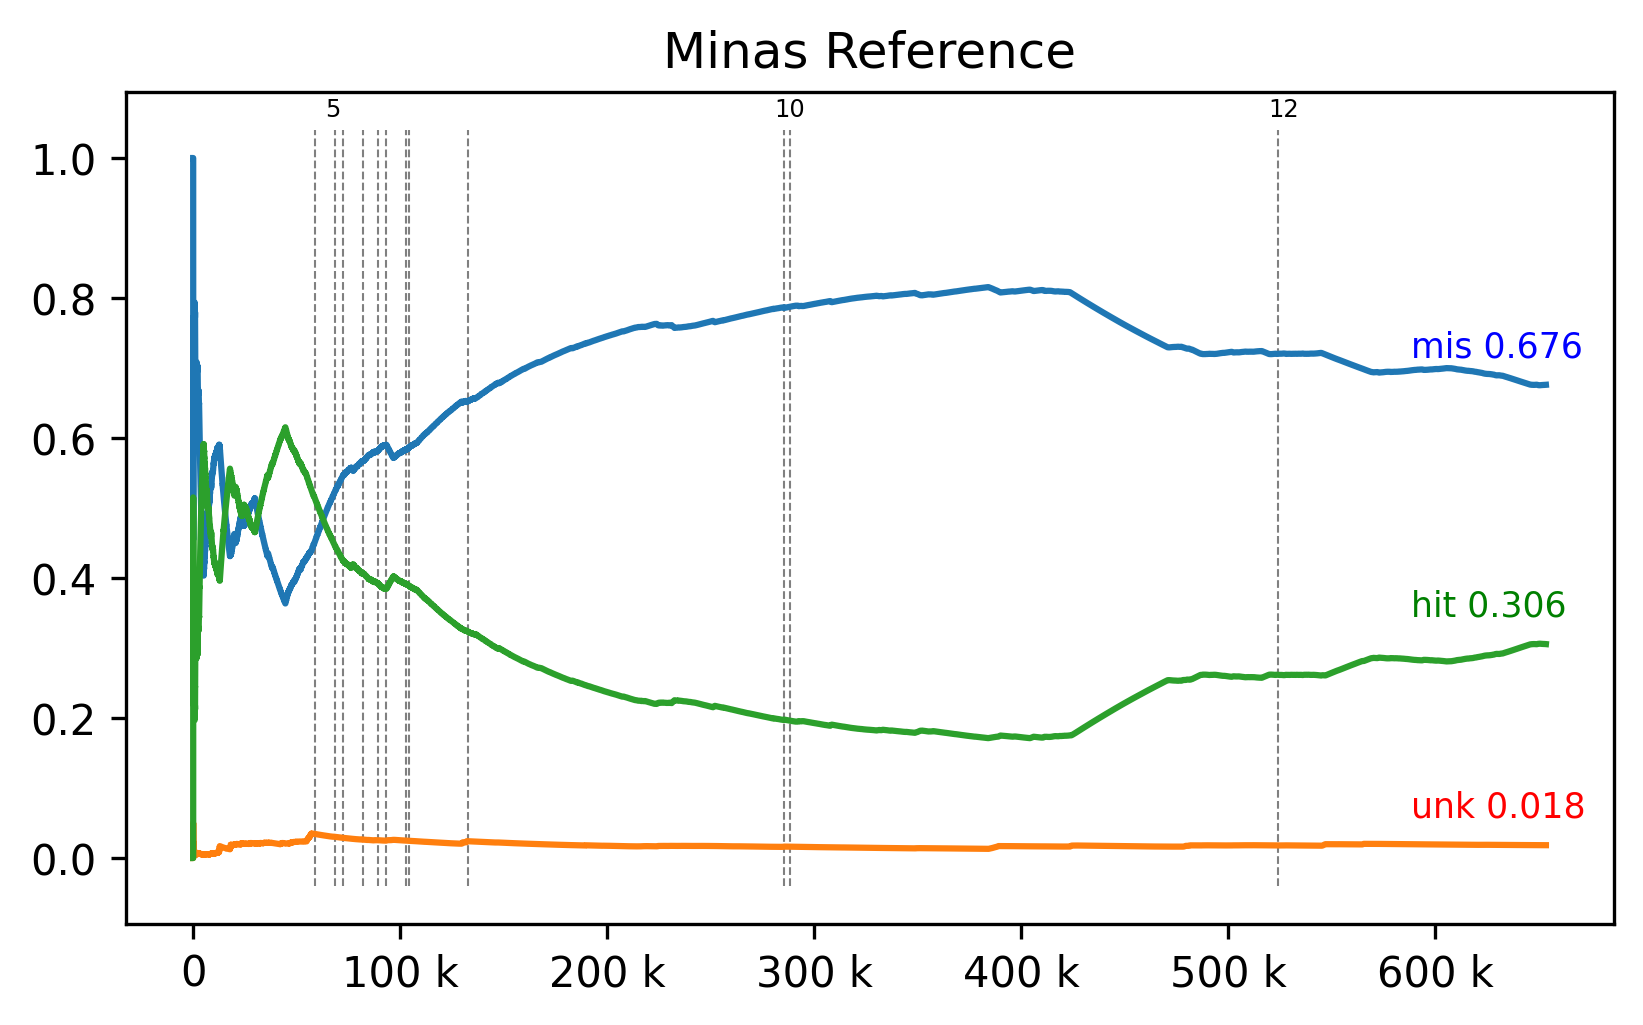
\includegraphics[width=1\linewidth]{experiments/revised-java-log.png}
    % \caption{Reference Implementation}
    \legend{Reference Implementation}
    \label{fig:validation-sub-java}
  \end{minipage}
  \hfill
  \begin{minipage}{0.48\textwidth}
    \centering
    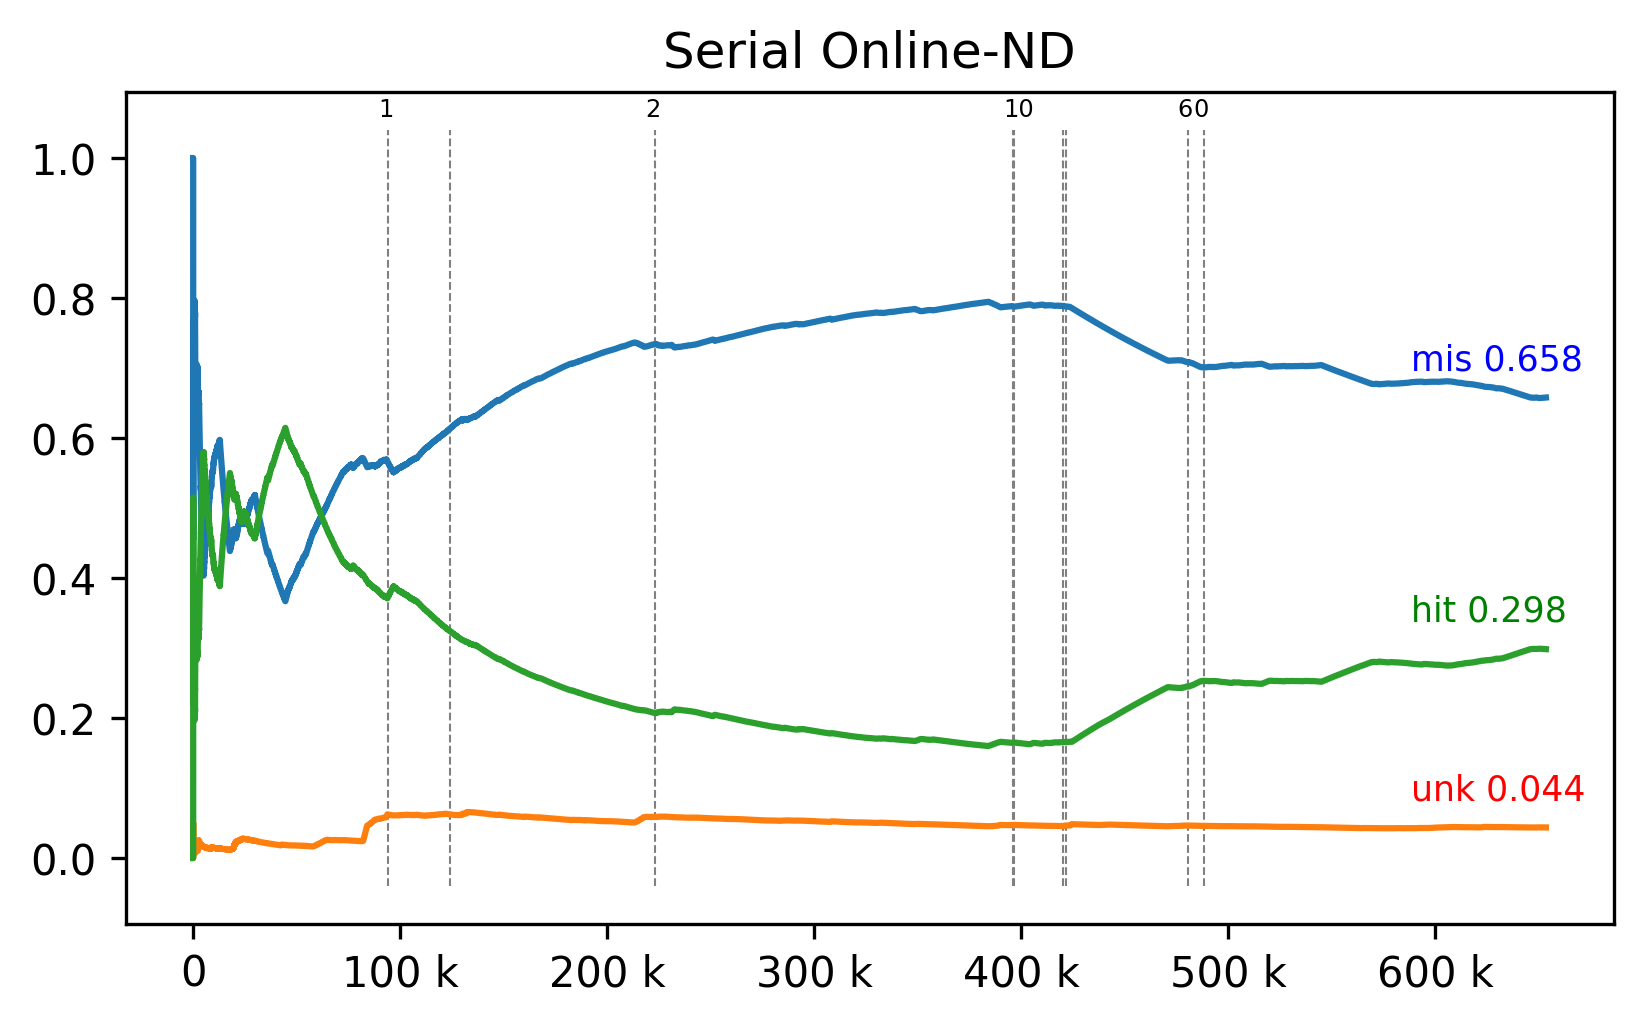
\includegraphics[width=1\linewidth]{experiments/online-nd-log.png}
    \caption{Serial Implementation}
    \label{fig:validation-sub-serial}
  \end{minipage}
  \vspace{5mm}
  \begin{minipage}{0.48\textwidth}
    \centering
    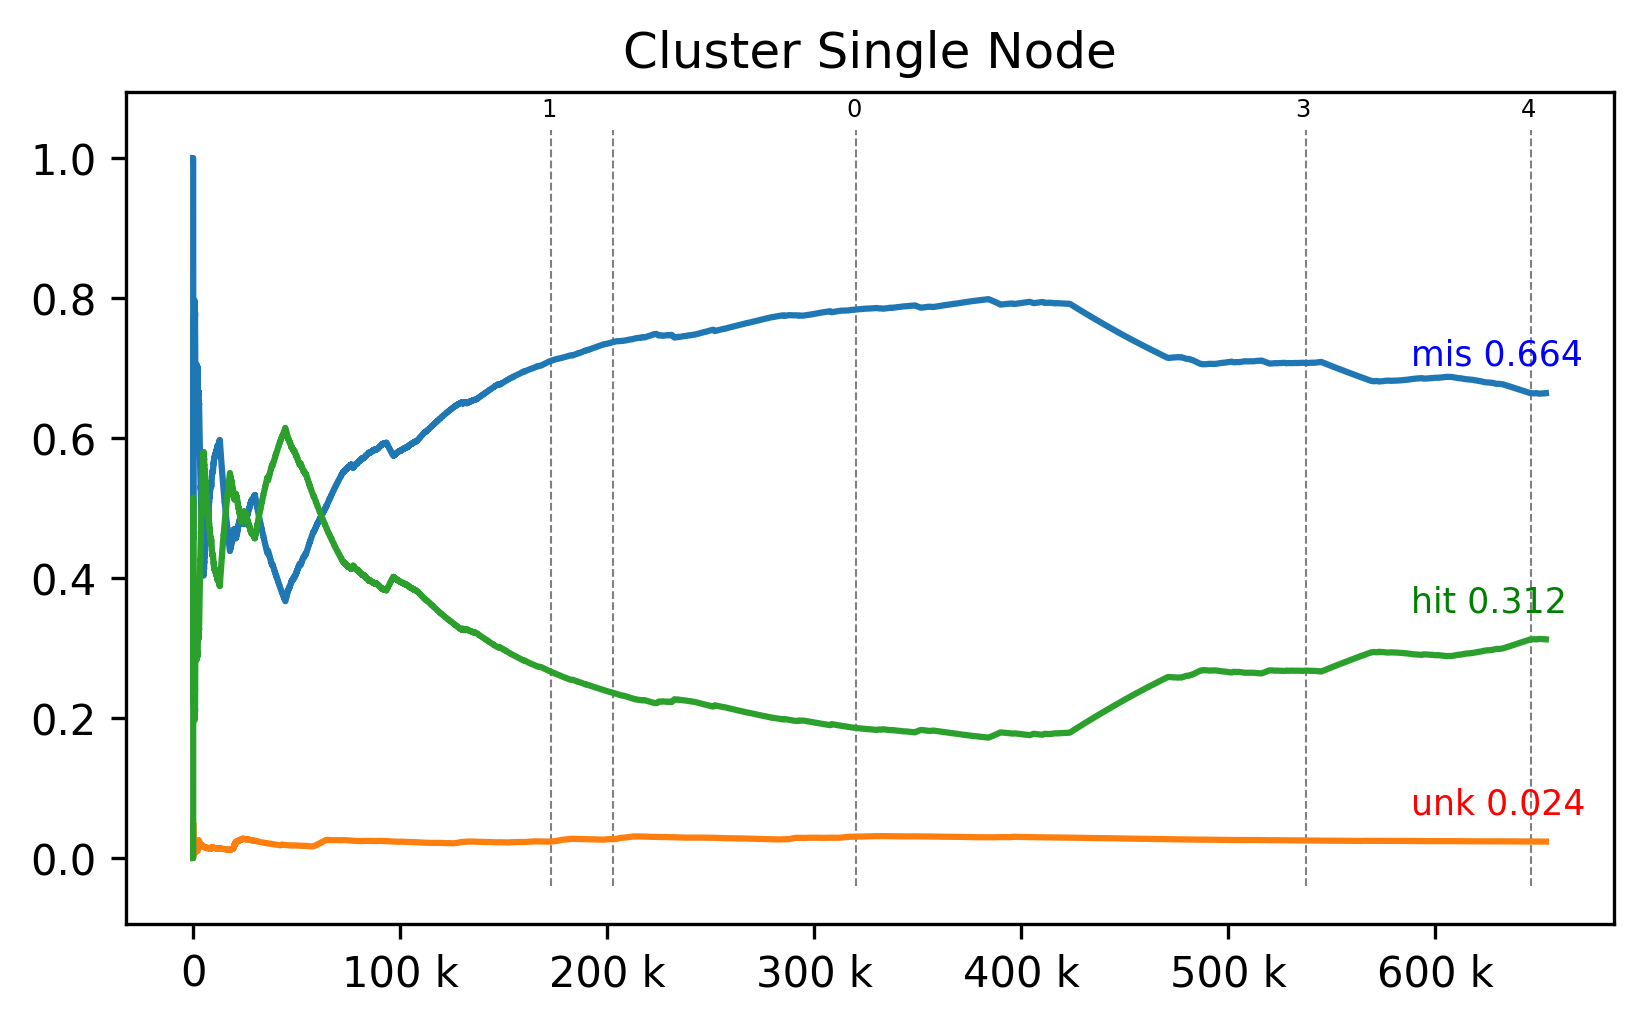
\includegraphics[width=1\linewidth]{experiments/tmi-base-log.png}
    \caption{Parallel single-node}
    \label{fig:cluster-sub-single}
  \end{minipage}
  \hfill
  \begin{minipage}{0.48\textwidth}
    \centering
    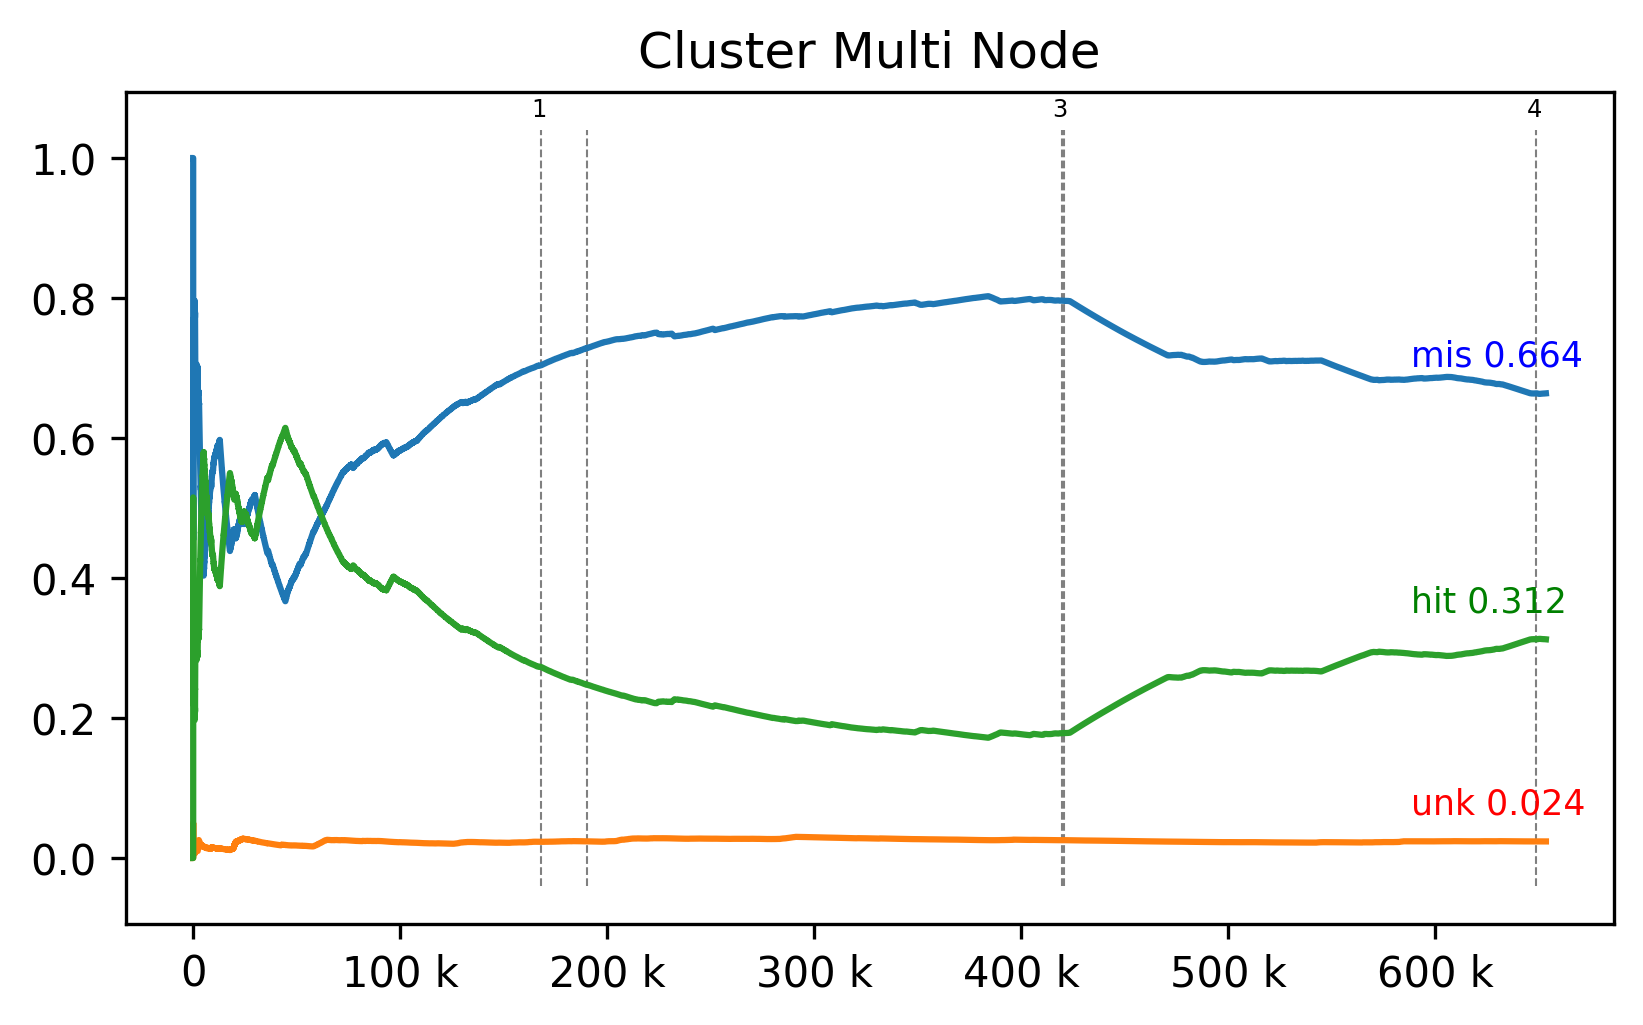
\includegraphics[width=1\linewidth]{experiments/tmi-n12-log.png}
    \caption{Parallel multi-node}
    \label{fig:cluster-sub-multi}
  \end{minipage}
  \caption{Stream hits and novelties visualization}
  \label{fig:visualization}
\end{figure}


\section{Conclusão}
\label{sec:exp-conclusao}

Portanto ... \todo{fix-me}
